\documentclass[11pt]{extarticle}
%\usepackage[margin=50pt]{geometry}
\usepackage{amsmath}
\usepackage[slovak]{babel}
\usepackage[T1]{fontenc}
\usepackage{multicol}
\usepackage{graphicx}
\usepackage{caption}
\graphicspath{ {../assets/} }
\usepackage{tikz}
\usepackage{pgfplots}
\pgfplotsset{
	table/search path={../assets/},
}

\title{%
Laboratórna práca č.2\\
Kmitavý pohyb
}
\author{}
\date{}

\begin{document}
	\maketitle
	\large
	\begin{tabular}{ll}
		Dátum merania: 7.2.2023 \hfill &Meno: Adam Labuš \\
		Spolupracovníci: Ivan Cabaj, Samuel Gereg, Andrej Blažek &Trieda: Sexta B \\
	\end{tabular}
	\vspace{50pt}
\section{Postup}
\begin{enumerate}
	\item Importneme video kmitajúce sa telesa do trackeru
	\item Nastavíme rozsah klipu - teda nastavíme štartovnú a konečnú snímku
	\item Nastavíme mierku podľa tyče, ktorá drží aparatúru
	\item Ideme na prvú snímku, a vyberieme si miesto na kmitavom telese, ktoré budeme trackovať. V našom prípade to bolo miesto, kde sa dotýkali háčiky dvoch závažií
	\item Pridáme súradnicovú os na miesto, ktoré budeme trackovať, tak aby prvý bod nášho tracku bol (0,0). Toto je presne, čo sme v našom meraní nespravili - náš prvý bod je (0,0)
	\item Trackujeme až po poslednú snímku
	\item Urobíme printscreen - \textit{Obr. 1}
	\item Nastavíme graf v závislosti $y$ od $t$ - \textit{Obr. 2}
	\item Ofitujeme daný graf - \textit{Obr. 3}
	\item Nastavíme pod seba grafy $t$ od $y$, $t$ od $v_y$ a $t$ od $a_y$ - \textit{Obr 4.}
\end{enumerate}
\section{Namerané a vypočítané hodnoty}
\subsection{Obrázky}
\begin{center}
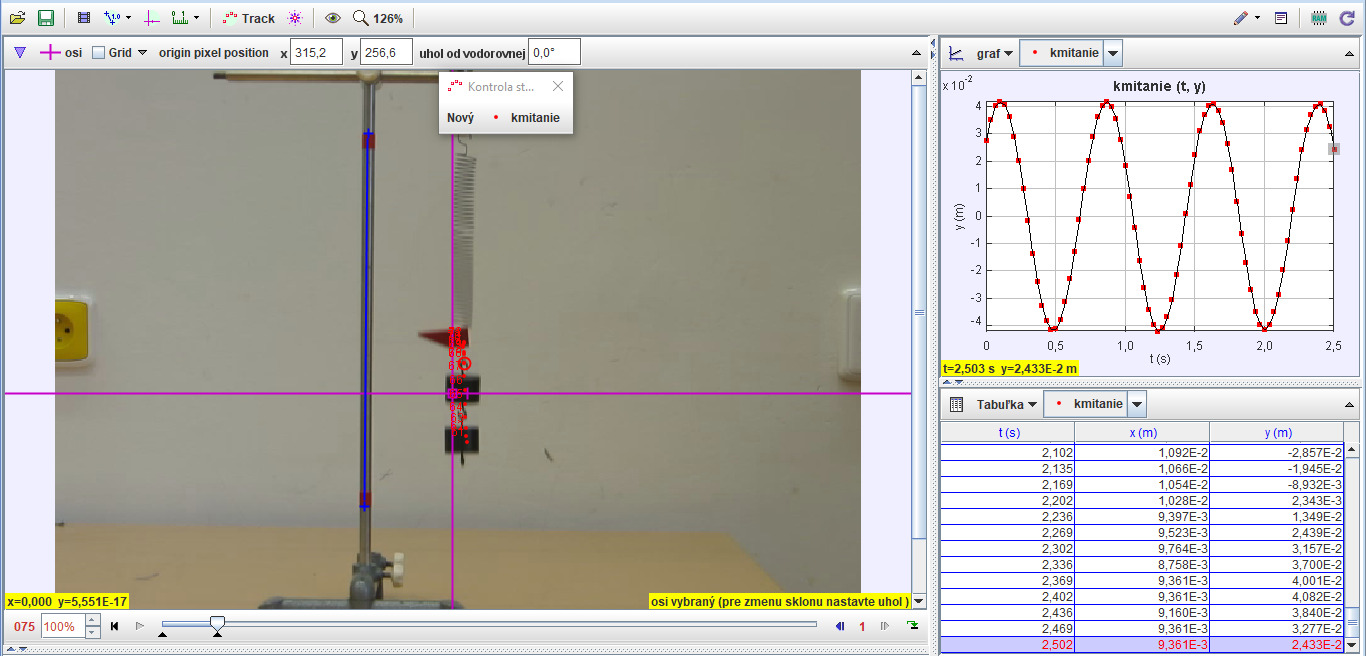
\includegraphics[width=.65\textwidth]{printscreen_po_merani}
\captionof{figure}{Printscreen po meraní}
\vspace{1.5em}
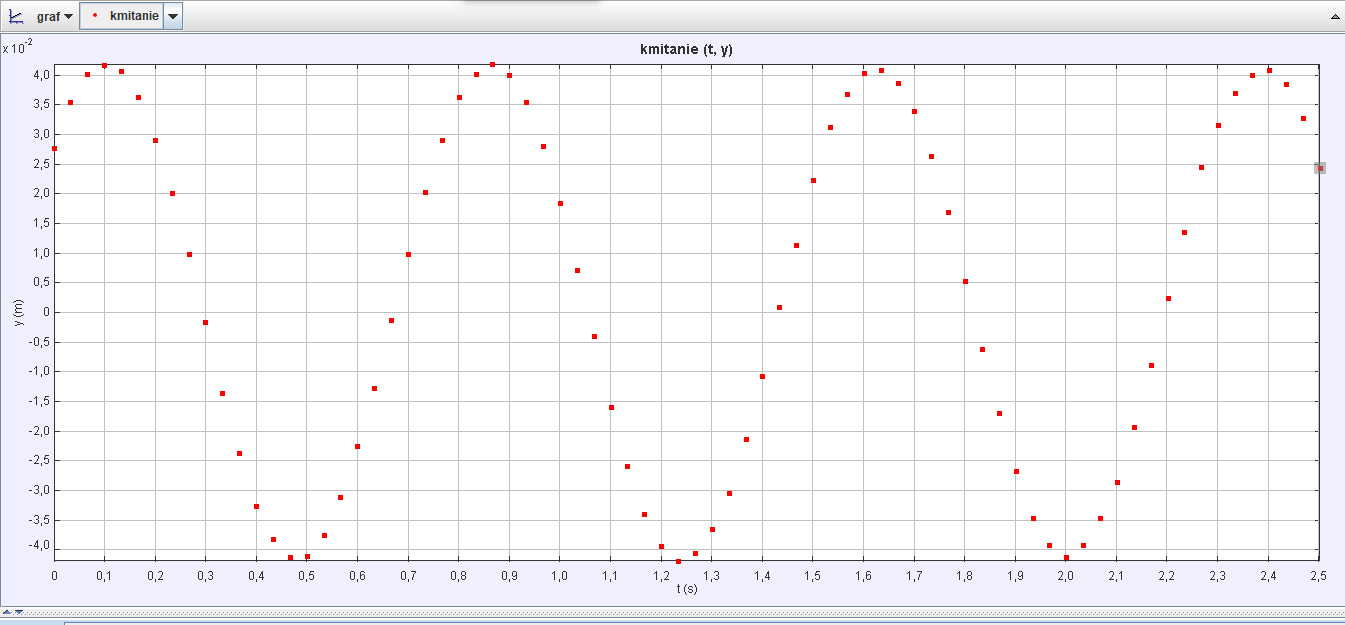
\includegraphics[width=.65\textwidth]{zakladny_graf}
\captionof{figure}{Graf závislosti $y$ od $t$}
\vspace{1.5em}
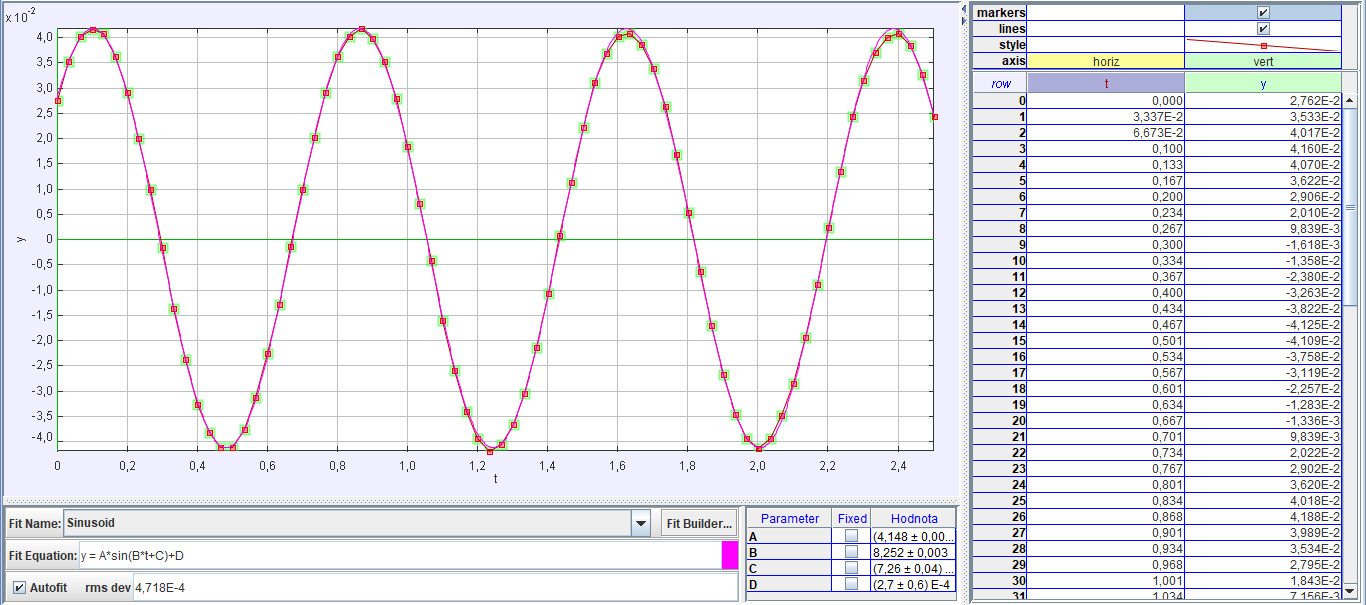
\includegraphics[width=.65\textwidth]{ofitovany_graf}
\captionof{figure}{Ofitovaný graf závislosti $y$ od $t$}
\vspace{1.5em}
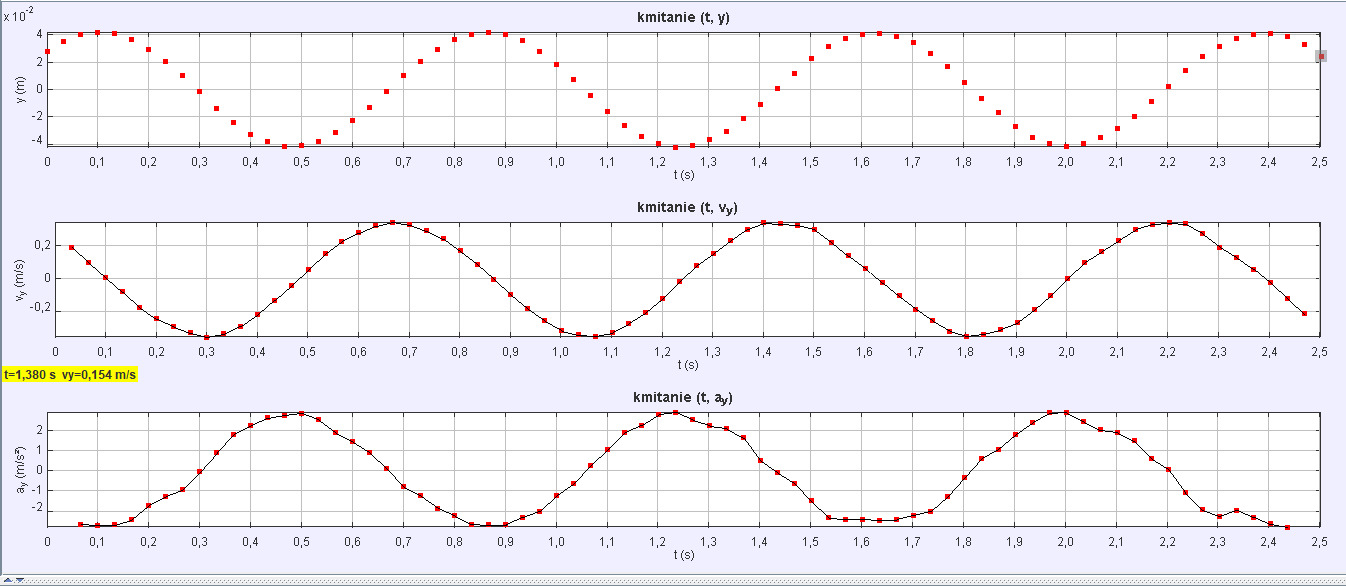
\includegraphics[width=.65\textwidth]{tri_grafy}
\captionof{figure}{Grafy $t$ od $y$, $t$ od $v_y$ a $t$ od $a_y$}
\end{center}

\subsection{Koeficienty ofitovanej funkcie}
Namerané hodnoty sme fitovali ku funkcií vo forme
\begin{center}
$f(x) = A*sin(Bx+C)+D$\\
$f(x) = 4.148*sin(8.252*x + 7.26) + 2.7*10^{-4}$
\end{center}

Pozn. $f(x)$ je v jednotke $m*10^{-2}$, teda centrimetroch\\[2em]

Tieto hodnoty si môžeme overiť manuálnymi výpočtami. Ako tieto koeficienty vypočítať je vidieť na tomto obrázku:\\
\begin{center}
	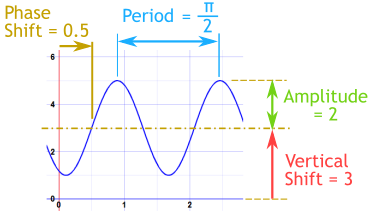
\includegraphics[width=0.5\textwidth]{fitovanie_sin}
	\captionof{figure}{Zdroj: \cite{obrazok}}
\end{center}


$A$, teda amplitúdu, vieme vypočítať nasledovne:
\begin{center}
$A = \frac{max_y - min_y}{2}$
\end{center}
''$A$'' sa rovná rozdielu medzi najvyššou hodnotou ''$y$'' a najnižšou hodnotou ''$y$'' deleno 2.\\
Dosadíme naše približné hodnoty.
\begin{center}
$A = \frac{4.1 - (-4.1)}{2}$\\
$A = 4.1$
\end{center}

$B$ je vyjadrenie periódy danej sinusoidy. Počíta sa nasledovne:
\begin{center}$B = \frac{2\pi}{p}$\end{center}
$p$ je perióda, teda horizontálna dĺžka jedného cyklu danej funkcie na grafe. Formálne, je to dĺžka na x-ovej osi medzi dvoma miestami, kde graf nadobúda tú istú hodnotu. Inač povedané je to dĺžka medzi dvoma vrcholmi na grafe. ...Inač povedané, je to čas kým teleso urobí jeden kmit.
Dosadenie naších hodnôt.
\begin{center}
$B = \frac{2\pi}{2 - 1.25}$\\
$B \approx 8.377$
\end{center}
Aký je súvis medzi periódou a frekvenciou? Frekvencia je len koľko periód prebehne za jednu sekundu, určuje sa jednotkou Hz. Takže keď je perióda jedna desatina sekundy, tak frekvencia je 10Hz. Frekvencia v našom meraní je približne 1.32Hz.
\\[2em]

$C$ je opak x-ového (horizontálneho) posunutia, takže $C = 5$ by posunulo celý graf do ľava o 5.
Ako bolo spomenuté, my sme v meraní nenastavili súradnicovú os na polohu trackovacieho bodu na prvej snímke, takže v našom grafe bude aj toto horizontálne posunutie. Podľa grafu vieme povedať, že je to približne:
\begin{center}
$C = 3$
\end{center}

$D$ je y-ové (vertikálne) posunutie.
V našom grafe je zanedbateľne malé:
\begin{center}
$D \approx 0$
\end{center}

\section{Záver}
Merali sme kmitavý pohyb, konkrétne telesa na pružine. Zistili sme, že keď zgrafujeme výšku tohto telesa v závislosti od času,
počas toho ako kmitá, tak dostaneme sinusoidu. Túto sme následne vyjadrili vzorcom:
\begin{center}$f(x) = 4.148*sin(8.252*x + 7.26) + 2.7*10^{-4}$\end{center}
Parametre sa rovnajú tým pádom:
\begin{center}
$A = 4.148$\\
$B = 8.252$\\
$C = 7.26$\\
$D = 2.7*10^{-4}$\\
\end{center}
Z \textit{Obr. 4} sme zistili nasledovné, keď $f(x)$ je sinsuoida tak prvá derivácia (rýchlosť) bude tiež sinsuoida, dokonca aj druhá derivácia je sinsuoida (zrýchlenie).
\begin{thebibliography}{3}
\bibitem{obrazok}
	https://www.mathsisfun.com/algebra/amplitude-period-frequency-phase-shift.html
\end{thebibliography}
\end{document}
